\section{Background: real-time neuroinformatics and control in behavioural systems
  neuroscience}

To understand the neural basis of behaviour, experiments need to control and quantify animal behaviour whilst recording, and often manipulating, neural activity. 
%
Powerful experimental designs require behavioural feedback (e.g.\ reward, lights, sounds, actuated
devices) or neural perturbation (e.g.\ using light-sensitive polarising
molecules) that depend on real-time behaviour or neural state.
%
Furthermore, it has become increasingly apparent that the neural signals that
drive complex behaviour are manifest in a broad population of neurons rather
than in single cells.  So current neural recording emphasises high-dimensional
signals from 100s to 1000s of neurons monitored using multi-electrode arrays or cellular-resolution imaging, with a wide array of probe configurations and neural targets.
%
This complexity of experiments limits the potential for database-driven progress in systems neuroscience.
%
The number of possible experiments is astronomical, and a new question must
usually be answered by designing and conducting a new experiment rather than
mining the data from an old one.

At present, progress in the field is held back by the challenge of rapidly designing and implementing new experimental protocols, and the difficulty of integrating state-of-the-art data processing and
neuroinformatics into custom experimental designs.
%
\textbf{Reproducibility}, in particular, depends on the availability of standardized tools for experimental control and analysis, shared between laboratories (Baker, 2016; Ioannidis, 2005). Although such tools exist in genetics, astronomy, physics and medicine (Fish et al., 2016; Abdalla et al., 2018, CERN Education, Communications and Outreach Group, 2018, Dickinson et al., 2016, Bycroft et al., 2018), they are mostly lacking in neuroscience, with documented consequences for the reliability of ``discoveries'' (Baker, 2016; Botvinik-Nezer et al., 2020; Button et al., 2013). 

\setlength{\columnsep}{1em}
\begin{wrapfigure}{r}{0.5\textwidth}
  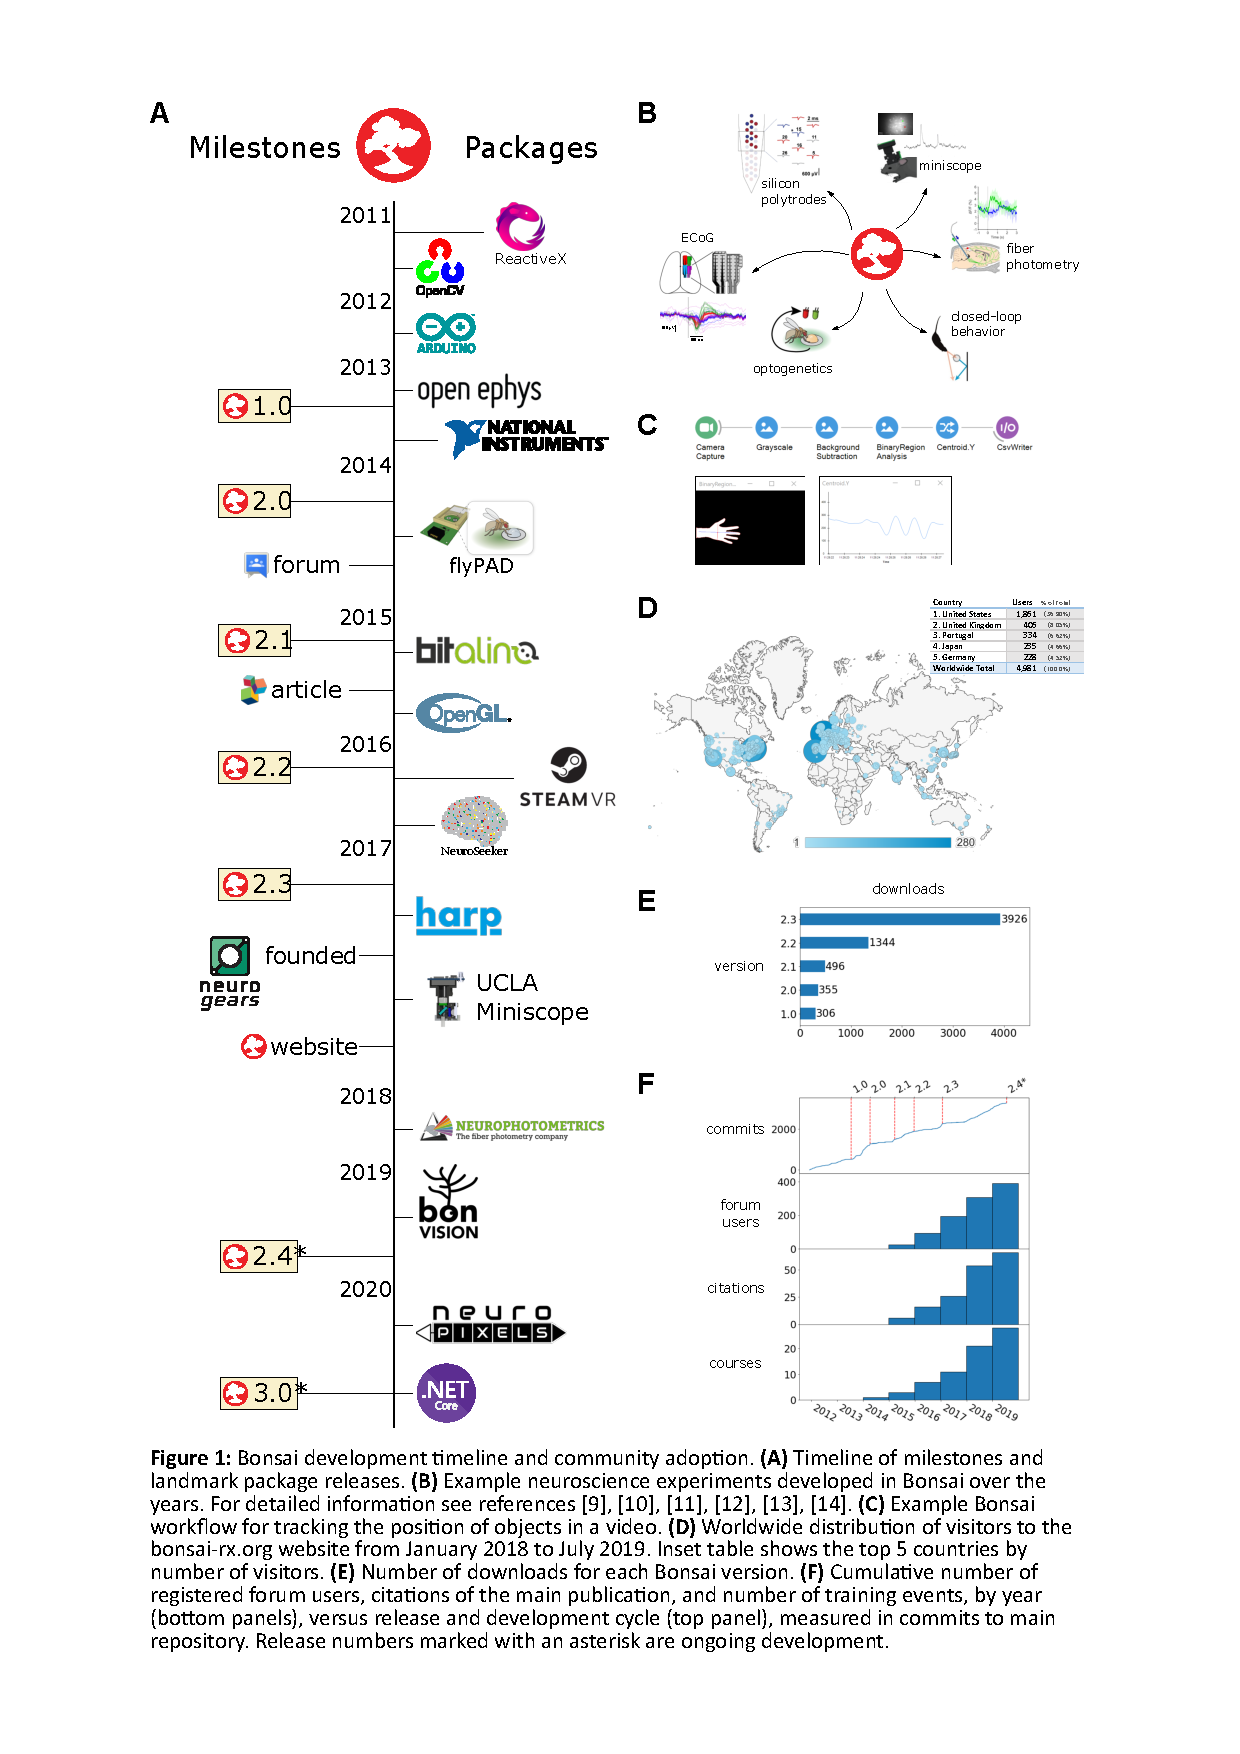
\includegraphics[width=0.5\columnwidth,viewport=65 50 500 800,clip]{figures/bonsai.pdf}
  \label{fig:bonsai}
\end{wrapfigure}

\textbf{Bonsai}~\citep{lopesEtAl15,lopesAndMonteiro21} is a free and open-source visual programming language developed 
in response to these challenges.
% ~\citep{lopesEtAl15,lopesAndMonteiro21} is a free and open-source visual
% programming language that 
Its design emphasises performance, flexibility, and ease-of-use,
allowing scientists with no previous programming experience to quickly develop
their own high-performance data acquisition and experimental control systems.
Bonsai combines a high-level event algebra for data streams with an integrated
development environment (IDE) and an extensive library of plugins supporting
multiple hardware and software packages used by the neuroscience research
community (Figure~\ref{fig:bonsai}A-B).
%
A Bonsai graphical program consists of one or more source data streams (e.g.\ neural activity, video, audio, sensors, etc)
and several interconnected operators that transform input to output
datastreams (Figure~\ref{fig:bonsai}C).

% I think we've said something similar in the first para  - m.
%
% Standard software tools for data analysis (ImageJ, MATLAB, R, etc.) have
% transformed progress inf increasingly “data-rich” sciences. However,
% equivalent standardised software tools for data acquisition and control of
% animal behaviour in neuroscience experiments are still lacking. Life science experiments demand
% a combination of multiple instrumentation and control technologies, for both
% behavioural and physiological investigations. The growing complexity on both the
% amount of data that is collected, and the rich conditions under which behaviour
% must be explored, place an increasing burden on experimenters to integrate
% highly specialised equipment in unique configurations, while often lacking
% expertise in the relevant engineering fields.



Bonsai has been adopted in hundreds of laboratories worldwide and has the largest user base in the systems neuroscience community (Figure~\ref{fig:bonsai}D-F).  In the last year alone, more than 1,000 new users incorporated Bonsai into their experimental protocols. The rapid rate of adoption of Bonsai in non-programmer experimental
labs highlights the need for accessible design tools that enable
state-of-the-art technology but also allow researchers to stay in control and flexibly
change their experimental paradigms.  Many open-source software tools are
either inaccessible to non-programmers, or too constrained to be of general use
outside their narrow domain of application. Bonsai has been successful because
it bridges this gap.

Bonsai also supports the growing wave of foundational
open hardware initiatives, such as OpenEphys \citep{siegleEtAl17} and UCLA
Miniscope~\citep{caiEtAl16}, allowing these tools to be quickly combined and integrated into new experiments~\citep{buccinoEtAl18}.
%
Bonsai has been adopted in large neuroscience undertakings like the
International Brain
Laboratory \footnote{internationalbrainlab.com/}
and the Allen Institute for Brain
Science\footnote{https://alleninstitute.org/what-we-do/brain-science/}.
%
Key to the wide adoption is the reproducibility that Bonsai ensures.  Data acquisition and experimental control protocols can be 
replicated in any laboratory just by sharing a Bonsai configuration file. 
%
% LEAVE OUT FOR THIS GRANT:
% More recently, Bonsai has started to expand outside the domain of neuroscience
% into biomedical research and biotechnology tool development, and even outside
% academia into public outreach and education programs.




Our proposed enhancements will \textbf{enhance, reinforce and support this key neuroinformatics
  resource to streamline reproducible experimental design, data collection and analysis, while making standardised implementations of cutting-edge machine-learning methodologies widely available to the community}, potentially creating the most powerful experimental
control and analysis tool available to neuroscientists, psychologists and
ethologists worldwide.

\subsection*{Other resources in the subject area}

The space of technologies serving experimental control and behaviour monitoring
is large, and is traditionally occupied either by domain-specific graphical
user interfaces for control and recording of specific devices and experiment
types (e.g.\ Open Ephys
GUI\footnote{https://open-ephys.org/gui/},
Miniscope DAQ
Software\footnote{https://github.com/Aharoni-Lab/Miniscope-DAQ-QT-Software})
or by real-time control frameworks for specifying task logic using state
machine or similar formalisms (e.g. NIMH ML\footnote{https://monkeylogic.nimh.nih.gov/},
pyControl\footnote{https://pycontrol.readthedocs.io/en/latest/},
Autopilot\footnote{https://docs.auto-pi-lot.com/en/latest/},
Sanworks\footnote{https://sanworks.io/index.php}).
These dedicated interfaces are typically very comfortable for experimenters
operating within the specific domain that the tool is designed for, but tend to
become unwieldy when there is a need to introduce a new device or variation of
a task which is outside the scope of the framework. The alternative is to use a
more general programming language like Python or MATLAB, with the disadvantage
of the code being harder to understand, maintain, and change. Programming
languages like LabVIEW straddle the middle ground and provide a high-level and
flexible visual interface for composing data acquisition and control systems
themselves. Unlike Bonsai, however, the graphical elements of LabVIEW are
heterogeneous and very fine grained, creating the need for long and complicated
logical structures to implement even a simple experimental control system. By
providing an extremely simple, yet flexible, visual syntax, Bonsai opens the
opportunity even for complete non-programmers to design and successfully
customize relatively complex experiments from the ground up. It is mostly this
capability which has made Bonsai so attractive as a standard tool in
experimental neuroscience.




%

%




% This resource will be built on the platform established by \textbf{Bonsai}.
%


% an established
% experimental control software ecosystem with a long development history and a
% large user base in systems neuroscience (Figure~\ref{fig:bonsai}).

% \subsection{Bonsai}
% \label{sec:bonsai}
%
% We will 
% 
% 
% 
% A central goal of the software resource proposed here is to address this
% problem, by extending Bonsai~(an experimental control software ecosystem;
% Figure~\ref{fig:bonsai} and Section~\ref{sec:bonsai}) with state-of-the-art
% online (and offline) data analysis methods
% (Figure~\ref{fig:proposedBonsaiExtensions} and
% Section~\ref{sec:functionality}).
% Bonsai is unique amongst experimental control systems in that
% it allows users with no programming expertise to design and implement
% sophisticated experiments.
%
% The latest Its large and rapidly growing community of users demonstrates the demand for such software resources.
%

% With the proposed enhancements, users of Bonsai will be able to use sophisticated \textbf{machine-learning methods} to
% control their experiments and analyse their data. This \textbf{democratisation}
% of machine learning functionality will allow scientists without computational
% skills to control sophisticated experiments and analyse their data in
% unprecedented ways, which will facilitate \textbf{advances in explaining how the
%   brain gives rise to behaviour}.



% \subsection{Bonsai}
% \label{sec:bonsai}

